\documentclass[11pt,a4paper]{article}

%============================%
%        BASIC PACKAGES      %
%============================%
\usepackage[a4paper,margin=3cm]{geometry}
\usepackage[T1]{fontenc}
\usepackage[utf8]{inputenc}
\usepackage[english]{babel}
\usepackage{lmodern}          % Better serif font
\usepackage{microtype}        % Better spacing and justification
\usepackage{parskip}          % Paragraph spacing instead of indentation
\usepackage{setspace}
\usepackage{hyperref}
\usepackage{datetime}
\newdateformat{monthyear}{\monthname[\THEMONTH] \THEYEAR}
\date{\monthyear\today}
\usepackage{graphicx}

%============================%
%        HEADINGS            %
%============================%
\usepackage{titlesec}
\renewcommand{\thesection}{\arabic{section}}    %all arabic is standard
\renewcommand{\thesubsection}{\arabic{section}.\arabic{subsection}}

% enumerate settings
\usepackage{enumitem}                           % for the [resume] option
\renewcommand{\theenumi}{\arabic{enumi}}        %options are {arabic, alph, Alph, roman, Roman}
\renewcommand{\theenumii}{\alph{enumii}}
\renewcommand{\theenumiii}{\roman{enumiii}}

%============================%
%        MATHEMATICS         %
%============================%
\usepackage{amsmath,amssymb,amsthm}
\usepackage{dsfont}
\renewcommand{\P}{\mathbb{P}}
\newcommand{\N}{\mathds{N}}
\newcommand{\Z}{\mathds{Z}}
\newcommand{\Q}{\mathds{Q}}
\newcommand{\R}{\mathds{R}}
\newcommand{\C}{\mathds{C}}
\newcommand{\EX}{\mathbb{E}}
\newcommand{\PP}{\mathcal{P}}           % power set
\newcommand{\ndiv}{\nmid}
\newcommand{\eps}{\varepsilon}
\let\temp\phi                           % varphi to phi
\let\phi\varphi
\let\varphi\temp
%different set notations
\newcommand{\sub}{\subset}              % new command to refer to standard notation \subset for standard subset (which might be equal)
\newcommand{\subneq}{\subsetneq}        % new command to refer to standard notation \subsetneq for proper subset (not allowed to be equal)
%\renewcommand{\sub}{\subseteq}         % use \subseteq instead of \subset for standard subset (which might be equal)
%\renewcommand{\subneq}{\subset}        % use \subset instead of \subsetneq for proper subset (which is not allowed to be equal)
%\renewcommand{\setminus}{-}            % use - instead of \ for relative complement of sets
%\renewcommand{\neg}{{\sim}}            % use ~ as negation symbol
\newcommand\norm[1]{\lVert#1\rVert}     % norm with double vertical lines
\newcommand\normx[1]{\Vert#1\Vert}      
\newcommand{\bigO}{\mathcal{O}}         % big O notation

%============================%
%        CODE BLOCKS         %
%============================%
\usepackage{minted}
\usemintedstyle{perldoc}
\setminted[haskell]{
  fontsize=\small,
  baselinestretch=1.05,
  frame=leftline,
  rulecolor=\color{black!70},
  framesep=2mm,
  linenos=false,
  tabsize=2,
  breaklines=true,
  autogobble=true
}

%============================%
%         TITLE INFO         %
%============================%
\title{\textbf{MSO Lab Assignment 2:\\
Programming Learning App}}
\author{Jan Huls (4699610), Arwin Moormans (4965957)}


\begin{document}
\maketitle
\section*{Software Design \& Patterns}
Below you will find a Class diagram to show the structure of the application.

\begin{figure}[htbp]\label{fig:class-diagram}
  \centering
  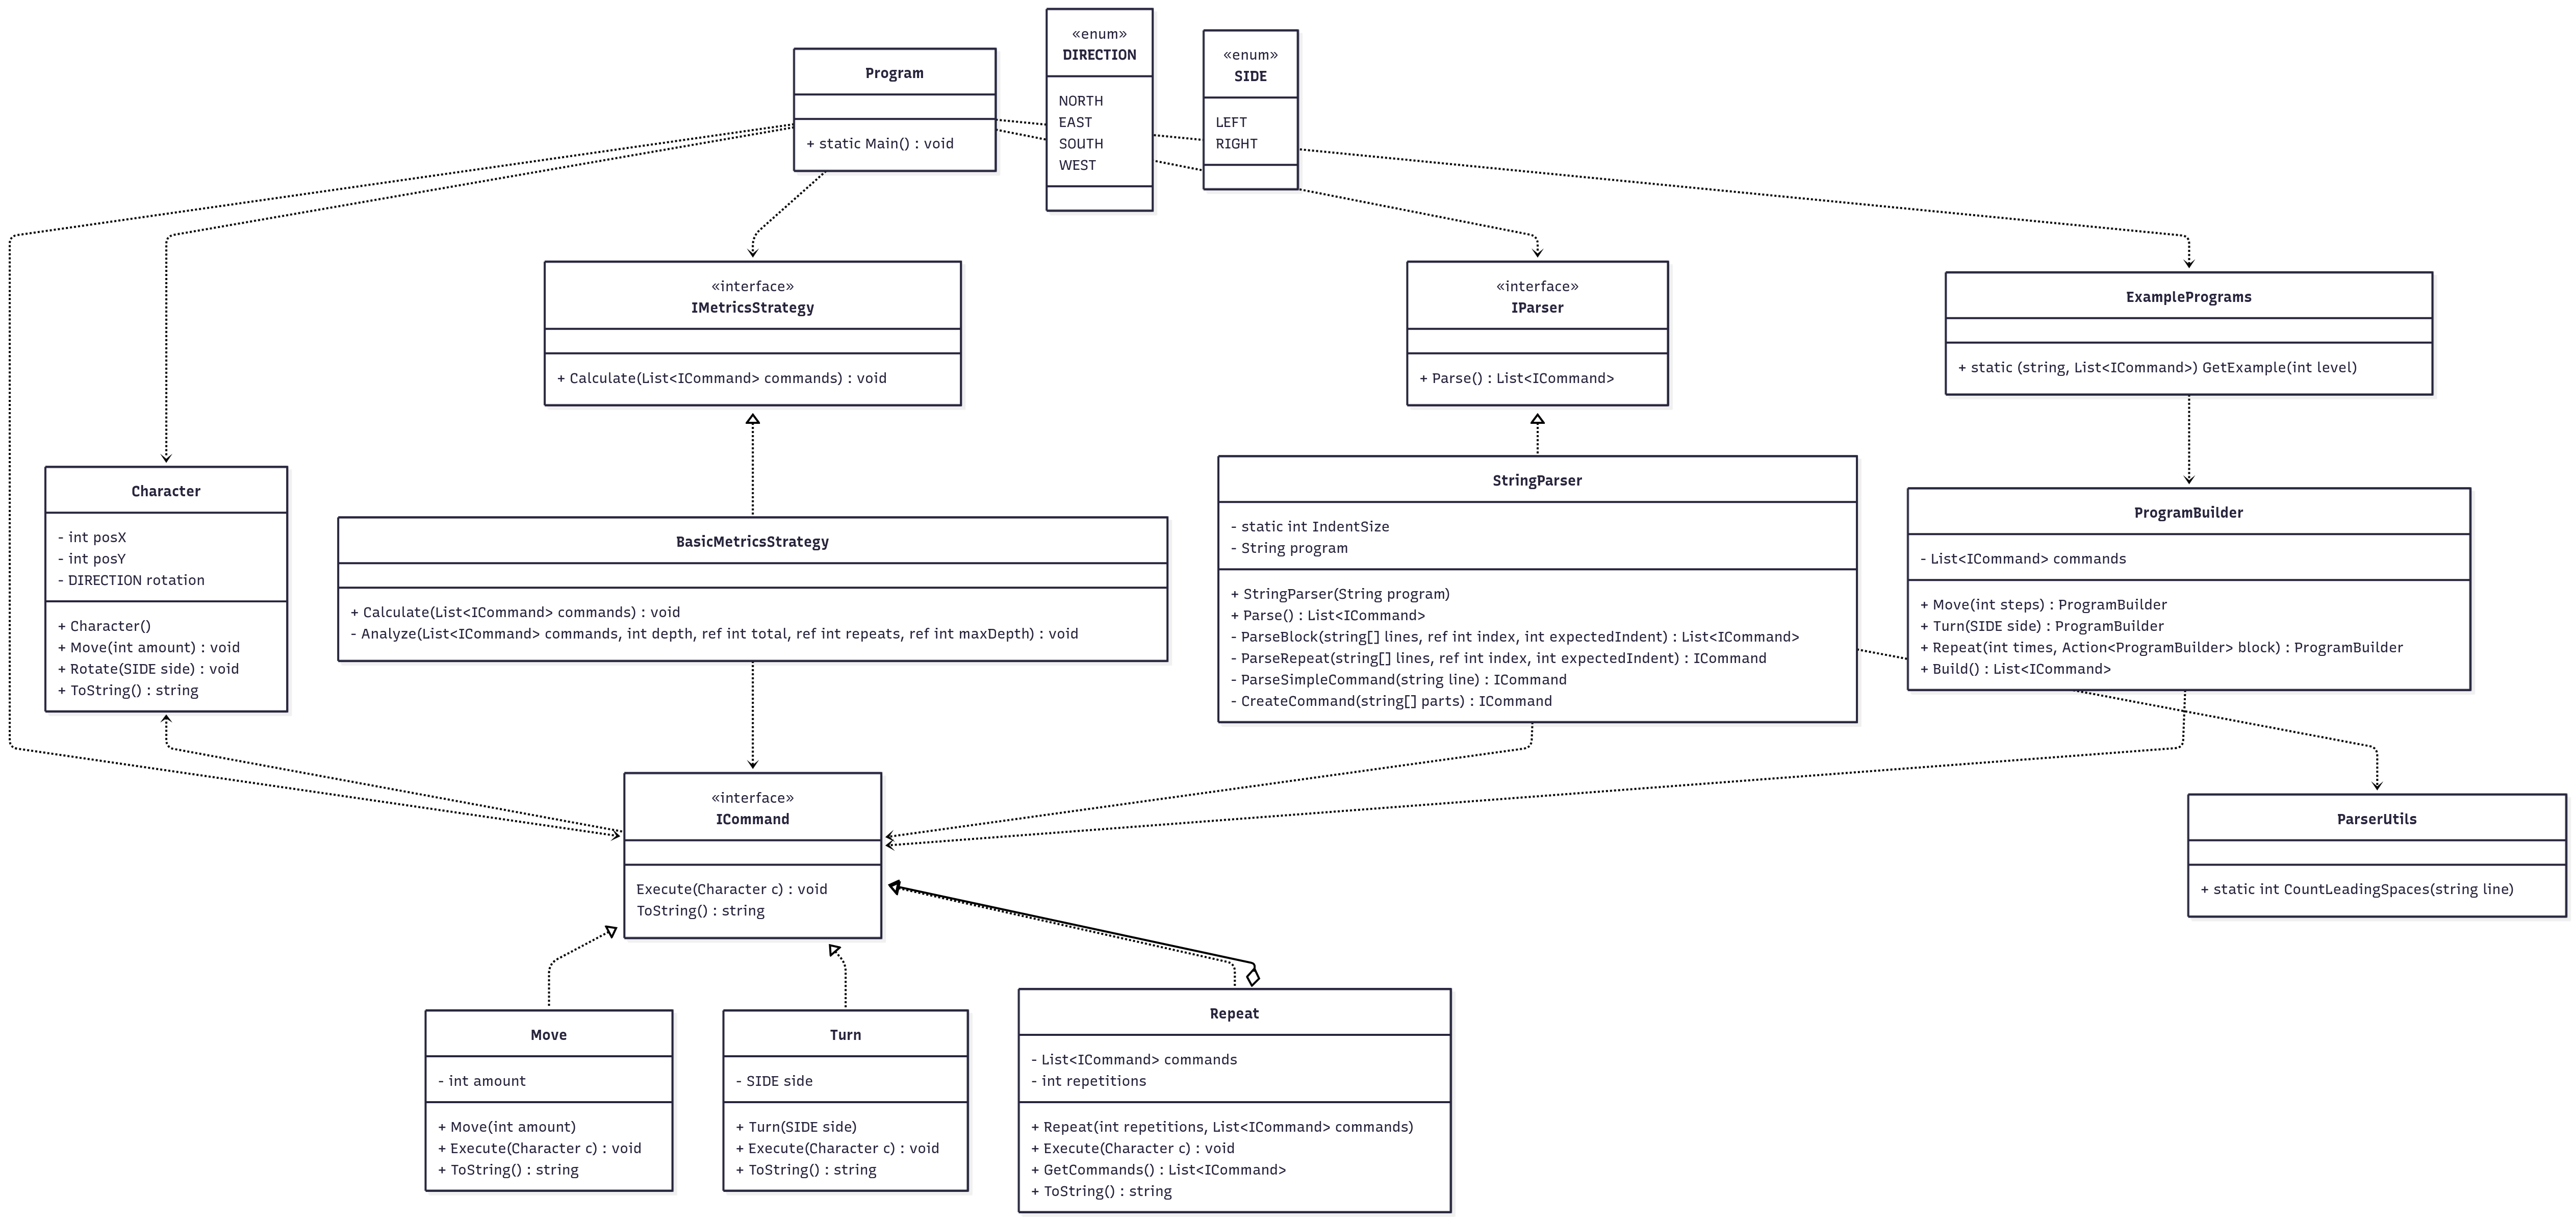
\includegraphics[width=0.9\textwidth]{class_diagram.png}
  \caption{Class diagram of the Programming Learning App}
\end{figure}
%hier die toevoegen kwee nie hoe da moet
We have used multiple patterns to structure our program.
The first pattern is the Composite pattern in the repeat command class.
This class holds all the functionality of the repeat command, such as the commands it needs to reapeat and how many times.
Because one of the repeated commands can be another reapeat command, we use the Composite pattern.
This makes a tree like structure where non-repeat commands are leafs and other repeat commands are nodes.
This way it is possible to call the Execute function of the root command and that will automaticly execute every command in the tree.

An other pattern is the Factory pattern that we use to construct commands bla bla 

For calculating different metrics we use the Strategy pattern.
This ensures that it is possible to add more 

At last we have used the Builder pattern to create the example programs.
This way it is possible to create 
%mis is deze ook niet nodig?? soort van wrm doen we nii gwn alle commands met de hand aan n lijst toevoegen
% anders moeten we ook deze class aanpassen elke keer als we commando toevoegen


%Composite pattern bij Repeat
%Factory pattern bij CommandFactory
%Strategy pattern bij MetricsCalculator, IMetricsStrategy
%Builder pattern bij ProgramBuilder

\section*{Evaluation}

\section*{Work Distribution \& Retrospective}

\end{document}